% Pengaturan ukuran teks dan bentuk halaman dua sisi
\documentclass[12pt]{report}

% Pengaturan ukuran halaman dan margin
\usepackage[a4paper,top=30mm,left=30mm,right=20mm,bottom=25mm]{geometry}

% Pengaturan ukuran spasi
\usepackage[singlespacing]{setspace}

% Pengaturan caption untuk tabel
\usepackage{caption}

% Judul dokumen
\title{Proposal Tugas Akhir ITS}
\author{Tanhar, Aaron Christopher}

% Pengaturan detail pada file PDF
\usepackage[pdfauthor={\@author},bookmarksnumbered,pdfborder={0 0 0}]{hyperref}


% Pengaturan ukuran indentasi
\setlength{\parindent}{2em}

% Package lainnya
\usepackage{changepage}
\usepackage{etoolbox} % Mengubah fungsi default

% Pengaturan jenis karakter
\usepackage[utf8]{inputenc}

\usepackage[style=apa, backend=biber]{biblatex}
\usepackage{enumitem} % Pembuatan list
\usepackage{lipsum} % Pembuatan template kalimat
\usepackage{graphicx} % Input gambar
\usepackage{longtable} % Pembuatan tabel
\usepackage[table,xcdraw]{xcolor} % Pewarnaan tabel
\usepackage{eso-pic} % Untuk menggunakan background image di halaman
\usepackage{txfonts} % Font times
\usepackage{changepage} % Pembuatan teks kolom
\usepackage{multicol} % Pembuatan kolom ganda
\usepackage{multirow} % Pembuatan baris ganda
\usepackage{tabularx} % Untuk mengatur kolom, seperti grid pada CSS
\usepackage{wrapfig}

% Pengaturan format daftar isi, daftar gambar, dan daftar tabel
\usepackage[titles]{tocloft}
\setlength{\cftbeforechapskip}{1.5ex}
\setlength{\cftbeforesecskip}{1.5ex}
\setlength{\cftbeforetoctitleskip}{0cm}
\setlength{\cftbeforeloftitleskip}{0cm}
\setlength{\cftbeforelottitleskip}{0cm}
\renewcommand{\cfttoctitlefont}{\hfill\Large\bfseries} % command untuk membuat heading bold dan besar
\renewcommand{\cftaftertoctitle}{\hfill}
\renewcommand{\cftloftitlefont}{\hfill\Large\bfseries}
\renewcommand{\cftafterloftitle}{\hfill}
\renewcommand{\cftlottitlefont}{\hfill\Large\bfseries}
\renewcommand{\cftafterlottitle}{\hfill}

% Definisi untuk "Hati ini sengaja dikosongkan"
\patchcmd{\cleardoublepage}{\hbox{}}{
  \thispagestyle{empty}
  \vspace*{\fill}
  \begin{center}\textit{[Halaman ini sengaja dikosongkan]}\end{center}
  \vfill}{}{}

  % Pengaturan penomoran halaman
\usepackage{fancyhdr}
\fancyhf{}
\renewcommand{\headrulewidth}{0pt}
\pagestyle{fancy}
\fancyfoot[C,CO]{\thepage}
\patchcmd{\chapter}{plain}{fancy}{}{}
\patchcmd{\chapter}{empty}{plain}{}{}

% Pengaturan format judul bab
\usepackage{titlesec}
\renewcommand{\thesection}{\thechapter.\arabic{section}}
\titleformat{\chapter}[hang]{\centering\bfseries\large}{BAB\ \arabic{chapter}\ }{0ex}{\vspace{0ex}\centering}
\titleformat*{\section}{\large\bfseries}
\titleformat*{\subsection}{\normalsize\bfseries}
\titlespacing{\chapter}{0ex}{0ex}{4ex}
\titlespacing{\section}{0ex}{1ex}{0ex}
\titlespacing{\subsection}{0ex}{0.5ex}{0ex}
\titlespacing{\subsubsection}{0ex}{0.5ex}{0ex}
\setcounter{secnumdepth}{3} % Untuk memberi penomoran pada \subsubsection

\counterwithin{figure}{chapter}
\counterwithin{table}{chapter}

% Mengganti figure dan table menjadi gambar dan tabel
\renewcommand{\figurename}{Gambar}
\renewcommand{\tablename}{Tabel}

% Tambahkan format tanda hubung yang benar di sini
\hyphenation{
  ro-ket
  me-ngem-bang-kan
  per-hi-tu-ngan
  tek-no-lo-gi
  me-la-ku-kan
  ber-so-si-al-i-sa-si
}

% Menambahkan resource daftar pustaka
\addbibresource{pustaka/pustaka.bib}

% Menyamakan indentasi list dengan paragraf
\setlist[]{labelindent=\parindent, align=left, leftmargin=*}

% Pengaturan format potongan kode
\usepackage{listings}
\definecolor{comment}{RGB}{0,128,0}
\definecolor{string}{RGB}{255,0,0}
\definecolor{keyword}{RGB}{0,0,255}
\lstdefinestyle{codestyle}{
  commentstyle=\color{comment},
  stringstyle=\color{string},
  keywordstyle=\color{keyword},
  basicstyle=\footnotesize\ttfamily,
  numbers=left,
  numberstyle=\tiny,
  numbersep=5pt,
  frame=lines,
  breaklines=true,
  prebreak=\raisebox{0ex}[0ex][0ex]{\ensuremath{\hookleftarrow}},
  showstringspaces=false,
  upquote=true,
  tabsize=2,
}
\lstset{style=codestyle}

% Isi keseluruhan dokumen
\begin{document}
% Nomor halaman pembuka dimulai dari sini
\pagenumbering{roman}

% Atur ulang penomoran halaman
\setcounter{page}{1}

% Sampul Bahasa Indonesia
\newcommand\covercontents{sampul/konten-id.tex}
\AddToShipoutPictureBG*{
  \AtPageLowerLeft{
    % Ubah nilai berikut jika posisi horizontal background tidak sesuai
    \hspace{-3.25mm}

    % Ubah nilai berikut jika posisi vertikal background tidak sesuai
    \raisebox{0mm}{
      
\includegraphics[width=\paperwidth,height=\paperheight]{sampul/gambar/sampul-luar-tipis.png}
    }
  }
}

% Menyembunyikan nomor halaman
\thispagestyle{empty}

% Pengaturan margin untuk menyesuaikan konten sampul
\newgeometry{
  top=65mm,
  left=30mm,
  right=30mm,
  bottom=20mm
}

\begin{flushleft}

  % Pemilihan font sans serif
  \sffamily

  % Pemilihan font bold
  \fontseries{bx}
  \selectfont
  \begin{spacing}{1.5}
    \input{\covercontents}
  \end{spacing}

\end{flushleft}

\restoregeometry


% Lembar pengesahan
\chapter*{LEMBAR PENGESAHAN}
%\begin{center}
%	\large
%  \textbf{LEMBAR PENGESAHAN}
%\end{center}

% Menyembunyikan nomor halaman
\thispagestyle{empty}

\begin{center}
  % Ubah kalimat berikut dengan judul tugas akhir
  \textbf{SISTEM BERBAGI DATA BERBASIS \emph{BLOCKCHAIN} UNTUK \emph{AUDIO PLAYER}
  DI \emph{METAVERSE}}
\end{center}

\begingroup
  % Pemilihan font ukuran small
  \small

  \begin{center}
    % Ubah kalimat berikut dengan pernyataan untuk lembar pengesahan
    \textbf{PROPOSAL TUGAS AKHIR} \\
    Diajukan untuk memenuhi salah satu syarat memperoleh gelar
    Sarjana Teknik pada 
    Program Studi S-1 Teknik Komputer \\
    Departemen Teknik Komputer \\
    Fakultas Teknologi Elektro dan Informatika Cerdas \\
    Institut Teknologi Sepuluh Nopember
  \end{center}

  \begin{center}
    % Ubah kalimat berikut dengan nama dan NRP mahasiswa
    Oleh: \textbf{Aaron Christopher Tanhar} \\
    NRP. 0721 19 4000 0055
  \end{center}

  \begin{center}
    Disetujui oleh Tim Penguji Proposal Tugas Akhir:
  \end{center}

  \begingroup
    % Menghilangkan padding
    \setlength{\tabcolsep}{0pt}

    \noindent
    \begin{tabularx}{\textwidth}{X c}
      % Ubah kalimat-kalimat berikut dengan nama dan NIP dosen pembimbing pertama
      Mochamad Hariadi, S.T., M.Sc., Ph.D.          & (Pembimbing) \\
      NIP: 19691209 199703 1 002                    & \\
      &  \\
      &  \\
      % Ubah kalimat-kalimat berikut dengan nama dan NIP dosen pembimbing kedua
      Dr. Surya Sumpeno, S.T., M.Sc.    & (Ko-Pembimbing) \\
      NIP: 19690613 199702 1 003        & \\
      % Ubah kalimat-kalimat berikut dengan nama dan NIP dosen penguji pertama
      Nama dosen penguji  & (Penguji I) \\
      NIP: 15640215 164201 1 001        & \\
      &  \\
      &  \\
      % Ubah kalimat-kalimat berikut dengan nama dan NIP dosen penguji kedua
      Nama dosen penguji  & (Penguji II) \\
      NIP: 18441015 190008 1 001        & \\
      &  \\
      &  \\
      % Ubah kalimat-kalimat berikut dengan nama dan NIP dosen penguji ketiga
      Nama dosen penguji            & (Penguji III) \\
      NIP: 19120623 195406 1 001        & \\
    \end{tabularx}
  \endgroup

  \vspace{4ex}

  \begin{center}
    % Ubah text dibawah menjadi tempat dan tanggal
    \textbf{SURABAYA} \\
    \textbf{Desember, 2022}
  \end{center}
\endgroup

\newpage

% Abstrak
\chapter*{ABSTRAK}

\begin{center}
  \textbf{SISTEM BERBAGI DATA BERBASIS \emph{BLOCKCHAIN} UNTUK \emph{AUDIO PLAYER}
    DI \emph{METAVERSE}}
\end{center}
\addcontentsline{toc}{chapter}{ABSTRAK}
% Menyembunyikan nomor halaman
\thispagestyle{empty}

\begin{flushleft}
  \setlength{\tabcolsep}{0pt}
  \bfseries
  \begin{tabular}{ll@{\hspace{6pt}}l}
    Nama Mahasiswa / NRP & : & Aaron Christopher Tanhar / 07211940000055 \\
    Departemen           & : & Teknik Komputer FTEIC - ITS               \\
    Dosen Pembimbing     & : & 1. Mochamad Hariadi, S.T., M.Sc., Ph.D.   \\
                         &   & 2. Dr. Surya Sumpeno, S.T., M.Sc.         \\
  \end{tabular}
  \vspace{4ex}
\end{flushleft}
\textbf{Abstrak}

% Isi Abstrak
Metaverse merupakan sebuah seperangkat ruang virtual, tempat seseorang dapat membuat dan menjelajah
dengan pengguna internet lainnya yang tidak berada pada ruang fisik yang sama dengan orang tersebut.
Pengaplikasiannya kerap kali menggunakan \emph{blockchain} sebagai solusi \emph{decentralized}. Metaverse sendiri
tentunya memerlukan adanya output audio, yang diwujudkan oleh Unreal Engine 5 dengan fitur metasoundnya.

Penggabungan keduanya dapat dicapai dengan menggunakan \emph{smart contract}. Maka di penelitian ini akan dibuat sistem yang dapat mewujudkan hal tersebut
dengan bantuan \emph{Ethereum Smart Contract}, NFT untuk menyimpan metadata, dan web3.storage IPFS untuk menyimpan file sumber audio untuk metasound.

Dengan adanya sistem terdesentralisasi tersebut juga diharapkan terwujudnya \emph{interoperability} agar metaverse ini dapat digunakan dan berkomunikasi dengan platform
blockchain lainnya.

\vspace{2ex}
\noindent
\textbf{Kata Kunci: \emph{Metaverse, Audio, Blockchain, Ethereum, NFT}}
\newpage

\chapter*{ABSTRACT}

\begin{center}
  \textbf{BLOCKCHAIN-BASED DATA SHARING SYSTEM FOR AUDIO PLAYER IN METAVERSE}
\end{center}
% Menyembunyikan nomor halaman
\thispagestyle{empty}

\begin{flushleft}
  \setlength{\tabcolsep}{0pt}
  \bfseries
  \begin{tabular}{lc@{\hspace{6pt}}l}
  Student Name / NRP&: &Aaron Christopher Tanhar / 07211940000055\\
  Department&: &Computer Engineering FTEIC - ITS\\
  Advisor&: &1. Mochamad Hariadi, S.T., M.Sc., Ph.D.\\
  & & 2. Dr. Surya Sumpeno, S.T., M.Sc.\\
  \end{tabular}
  \vspace{4ex}
\end{flushleft}
\textbf{Abstract}

% Isi Abstrak
The Metaverse is a set of virtual spaces, where one can create
and browse with other internet users who are not in the same physical space
with that person. The application often uses blockchain as a solution
decentralized. The Metaverse itself certainly requires an audio output, which is realized
by Unreal Engine 5 with its metasound feature.

Merging the two can be achieved by using smart contracts. Then in
This research will create a system that can make this happen with the help of Ethereum
Smart Contract, NFT to store metadata, and IPFS web3.storage to store
audio source files for metasound.

With the existence of a decentralized system, it is also hoped that interoperability will be realized.
ability to make this metaverse usable and communicate with other blockchain platforms.

\vspace{2ex}
\noindent
\textbf{Keywords: \emph{Metaverse, Audio, Blockchain, Ethereum, NFT}}
\newpage

\begin{spacing}{1.5}
  % Daftar isi
  \renewcommand*\contentsname{DAFTAR ISI}
  \addcontentsline{toc}{chapter}{\contentsname}
  \tableofcontents
  \newpage

  % Daftar gambar
  \renewcommand*\listfigurename{DAFTAR GAMBAR}
  \addcontentsline{toc}{chapter}{\listfigurename}
  \listoffigures
  \newpage

  % Daftar tabel
  \renewcommand*\listtablename{DAFTAR TABEL}
  \addcontentsline{toc}{chapter}{\listtablename}
  \listoftables
  \newpage
\end{spacing}

% Nomor halaman isi dimulai dari sini
\pagenumbering{arabic}

% Konten pendahuluan
\chapter{PENDAHULUAN}

\section{Latar Belakang}

% Ubah paragraf-paragraf berikut sesuai dengan latar belakang dari tugas akhir
Munculnya teknologi \emph{virtual reality (VR)} dan pengembangan platform metaverse telah mengarah pada terciptanya
pengalaman online yang imersif di mana pengguna dapat berinteraksi satu sama lain dan terlibat dalam berbagai aktivitas, apalagi setelah  Mark Zuckerberg
membeli oculus \parencite{luckerson2014facebook}.
Salah satu aktivitas tersebut adalah memainkan alat musik sebagai karakter virtual, yang dapat dicapai melalui penggunaan
teknologi motion capture dan simulasi instrumen virtual.

Namun, sistem saat ini untuk berbagi dan mengakses data musik di metaverse bersifat terpusat dan sering mengandalkan teknologi
hak cipta, yang dapat membatasi fleksibilitas dan interoperabilitas pengalaman musik. Pendekatan yang terdesentralisasi dan terbuka
untuk berbagi data dapat memungkinkan ekosistem musik yang lebih beragam dan interaktif di dalam \emph{metaverse}.

Salah satu fitur dari Unreal Engine 5 yaitu Metasound yang dapat melakukan pengolahan audio dengan mudah bagi para pengembang. Unreal Engine 5 juga
memiliki fitur yakni API blockchain sehingga dapat mengeksekusi \emph{smart contract}. Fitur ini dinamakan Web3.UE. Web3.Unreal adalah plugin
\emph{open source} yang dibuat untuk pengembang game dan komunitas untuk membantu mereka yang bekerja dengan Unreal Engine untuk mengintegrasikan
fungsionalitas blockchain ke dalam game mereka. Kedua hal ini dapat dikombinasikan dan digunakan untuk
pengembangan metaverse.

Metaverse telah digambarkan sebagai iterasi baru dari internet yang menggunakan headset VR, teknologi blockchain,
dan avatar dalam integrasi baru dunia fisik dan virtual. \parencite{DWIVEDI2022102542}. Dalam proposal penelitian ini, saya mengusulkan
untuk merancang dan mengimplementasikan sistem berbagi data berbasis \emph{blockchain}
untuk \emph{musical player} di metaverse dengan NFT. Sistem ini akan menggunakan smart contract dan solusi penyimpanan terdesentralisasi
untuk memungkinkan pengguna berbagi dan mengakses data musik dari metaverse dengan cara yang aman dan transparan.

\section{Rumusan Masalah}

% Ubah paragraf berikut sesuai dengan rumusan masalah dari tugas akhir
Di dunia \emph{virtual metaverse}, kebutuhan akan sistem yang aman dan efisien untuk berbagi data terkait musik semakin meningkat.
Saat ini, data ini sering disimpan dalam database terpusat yang rentan terhadap pelanggaran keamanan dan
penyensoran, dan dapat menyulitkan pengguna untuk mengakses dan mengontrol data mereka sendiri. Dibutuhkan juga sistem blockchain dengan interoperabilitas sehingga
pengembang metaverse dapat mengembangkan sistem yang dapat berkomunikasi dengan blockchain yang lainnya.

\section{Batasan Masalah}

% Ubah paragraf berikut sesuai dengan rumusan masalah dari tugas akhir
Untuk memfokuskan permasalahan yang diangkat maka dilakukan pembatasan ma-
salah. Batasan - batasan masalah tersebut diantaranya:
\begin{enumerate}
  \item Jenis \emph{Blockchain} yang digunakan adalah Ethereum.
  \item Target pengguna adalah pengguna metaverse.
  \item Target platform musik adalah Metasounds di Unreal Engine 5.
  \item Data berisi JSON yang adalah metadata yang diperuntukkan untuk metasound.
  \item File audio disimpan di IPFS
\end{enumerate}

\section{Tujuan Penelitian}

% Ubah paragraf berikut sesuai dengan tujuan penelitian dari tugas akhir
Penelitian ini memiliki tujuan untuk membuat sistem yang
dapat melakukan sharing data untuk musical player yang ada
di Metaverse menggunakan platfrom blockchain, agar
pengguna metaverse dapat menggunakan platform music
dan diintegrasikan dengan metasound.

\section{Manfaat}
Manfaat yang bisa didapat dari hasil tugas akhir ini adalah
memajukan pengembangan metaverse pada bidang audio dan sistem berbagi data blockchain
terkhususnya bagi para pengembang Web3.


% Konten tinjauan pustaka
\section{TINJAUAN PUSTAKA}

% Ubah konten-konten berikut sesuai dengan isi dari tinjauan pustaka

\subsection{Jaringan Terdistribusi}

Jaringan Terdistribusi adalah sebuah jaringan dimana setiap
node dalam cluster tersebut saling terhubung satu sama lain. Ja-
ringan desentralisasi mendistribusikan data, informasi, dan memp-
roses beban kerja di seluruh komputer yang berpartisipasi dalam
jaringan. Hal ini memungkinkan untuk toleransi kesalahan yang
lebih besar sebagai komponen kunci dari jaringan di distribusikan
di beberapa mesin, jika salah satu jaringan (hardware) down, maka
jaringan secara keseluruhan terus berfungsi.
Jaringan terdesentralisasi memiliki keuntungan lebih aman da-
ripada jaringan terpusat, tidak ada satu server pusat yang ditargetk-
an oleh penyerang. Jika seseorang ingin menyerang jaringan, mereka
perlu untuk menyerang beberapa node dalam jaringan. Karena ti-
dak ada kekuasaan dalam jaringan, pengguna bisa lebih memperca-
yai sistem, namun juga karena tidak ada kekuasaan dalam jaringan,
apabila ada masalah dalam jaringan tidak ada otoritas pusat yang
membantu menyelesaikan masalah hal ini yang membedakan anta-
ra jaringan terpusat dan jaringan terdistribusi.

\subsection{Metaverse}

Istilah metaverse pertama kali digunakan oleh Neal Stephenson di novelnya \emph{Snow Crash} untuk
mendeskripsikan dunia virtual dimana karakter protagonisnya, \emph{Hiro Protagonist}
, bersosialisasi, belanja, dan mengalahkan musuh-musuh dunia nyata melalui avatarnya. Ini bukanlah konsep yang baru
. Faktanya, film garapan Steven Spielberg pada tahun 2018 yang berjudul \emph{Ready Player One} juga mengambil konsep yang serupa dan
menggunakannya dengan sangat ciamik. Definisi teknis dari Metaverse itu sendiri adalah sebuah ruang virtual dimana orang-orang didalamnya bisa berinteraksi 
dengan lingkungan yang dibuat oleh komputer dan pemain lain.

\subsection{ERC-721}
ERC-721 merupakan antarmuka standar untuk membuat \emph{Non Fungible Token}, atau NFT.
Use case untuk NFT adalah kepemilikan asset digital dan transaksinya hingga pengiriman ke 
\emph{crypto wallet} pihak ketiga.

\subsection{Solidity}
Solidity adalah adalah bahasa tingkat tinggi berbasis objek untuk mengimplementasikan
\emph{smart contract}. Solidity ini dijalankan didalam Ethereum Virtual Machine (EVM).
Kontrak di Solidity mirip dengan class dalam bahasa object-oriented. Setiap kontrak dapat berisi pernyataan tentang :ref:`structure-state-variables`, :ref:`structure-functions`, :ref:`structure-function-modifiers`, :ref:`structure-events`, :ref:`structure-errors`, :ref:`structure-struct-types` dan :ref:`structure-enum-types`. Lebih jauh, kontrak dapat mewarisi dari kontrak lain.

Ada juga jenis kontrak khusus yang disebut :ref:`libraries<libraries>` dan :ref:`interfaces<interfaces>`.

Bagian tentang :ref:`kontrak<contracts>` berisi lebih banyak detail daripada bagian ini, yang berfungsi untuk memberikan gambaran singkat.

\subsection{Blockchain}

Blockchain adalah database terdistribusi yang digunakan un-
tuk menangani record data yang terus bertambah, record data ini
disebut dengan block. Setiap block memiliki penanda waktu dan ko-
de unik yang terhubung dengan block sebelumnya, sehingga masing
masing block tersebut saling terhubung satu sama lainnya dan ti-
dak bisa untuk diubah. Blockchain biasanya dikelola oleh jaringan
peer-to-peer yang secara kolektif mengikuti protokol untuk memva-
lidasi block baru. Jika terdapat perintah penambahan block baru,
maka setiap node pada jaringan peer-to-peer tersebut akan terlebih
dahulu memvalidasi block dan kemudian seluruh node akan mem-
perbarui record data miliknya [18]. Blockchain memiliki 3 type [19]
yaitu Public Blockchain yang dikembangkan secara bersama-sama
oleh publik dan siapa saja dapat ikut serta untuk mengembangk-
an blockchain, Private Blockchain yang hanya bisa digunakan oleh
organisasi tertentu, consortium blockchain yang dikembangkan oleh
suatu kelompok secara bersama untuk kepentingan tertentu, seder-
hananya blockchain konsorsium merupakan blockchain privat yang
diberdayakan oleh lebih dari satu kelompok.

\subsubsection{Unreal Engine 5}

Unreal Engine (UE) adalah Game Engine grafis komputer 3D yang dikembangkan oleh Epic Games, pertama kali dipamerkan dalam game penembak orang pertama tahun 1998 Unreal. 
Awalnya dikembangkan untuk penembak orang pertama PC, sejak itu telah digunakan dalam berbagai genre permainan dan telah diadopsi oleh industri lain, terutama industri film dan televisi. Ditulis dalam C++, 
Unreal Engine memiliki fitur portabilitas tingkat tinggi, mendukung berbagai platform desktop, seluler, konsol, dan virtual reality (VR).
Generasi terbaru, Unreal Engine 5, diluncurkan pada April 2022. Seperti pendahulunya yang dirilis pada Maret 2014, kode sumbernya tersedia di GitHub setelah mendaftarkan akun, dan penggunaan komersial diberikan 
berdasarkan model royalti. Epic membebaskan margin royalti mereka untuk game sampai pengembang memperoleh pendapatan US\$1 juta dan biaya tersebut dibebaskan jika pengembang menerbitkan di Epic Games Store. Epic telah memasukkan fitur dari perusahaan yang diakuisisi seperti Quixel di mesin, yang dipandang terbantu oleh pendapatan Fortnite.
Unreal Engine 5 terungkap pada 13 Mei 2020, mendukung semua sistem yang ada termasuk konsol generasi berikutnya PlayStation 5 dan Xbox Series X/S.\citep{StattEpicAnnounce} Pengerjaan mesin dimulai sekitar dua 
tahun sebelum diumumkan.\citep{DeanTakahashi} UE5 dirilis dalam early access pada 26 Mei 2021,\citep{EddieMakuch} dan secara resmi diluncurkan untuk pengembang pada 5 April 2022.\citep{UE5Launch}

Salah satu fitur utamanya adalah Nanite, mesin yang memungkinkan bahan sumber fotografi dengan detail tinggi diimpor ke dalam game.\citep{ValentineRebekah} Teknologi geometri tervirtualisasi Nanite memungkinkan Epic memanfaatkan akuisisi Quixel sebelumnya, perpustakaan fotogrametri terbesar di dunia pada 2019. Tujuan Unreal Engine 5 adalah untuk memudahkan pengembang 
membuat dunia game yang mendetail tanpa harus menghabiskan banyak waktu untuk membuat aset detail baru.\citep{DeanTakahashi} Nanite dapat mengimpor hampir semua representasi objek dan lingkungan tiga dimensi yang sudah ada sebelumnya, termasuk model ZBrush dan CAD, memungkinkan penggunaan aset berkualitas film.\citep{AndrewTarantola} Nanite secara otomatis menangani tingkat detail (LODs) 
dari objek yang diimpor ini sesuai dengan platform target dan jarak menggambar, tugas yang harus dilakukan oleh seorang seniman jika tidak.\citep{KyleOrland} Lumen adalah komponen lain yang digambarkan sebagai "solusi iluminasi global yang sepenuhnya dinamis yang segera bereaksi terhadap pemandangan dan perubahan cahaya". Lumen menghilangkan kebutuhan 
seniman dan pengembang untuk membuat peta cahaya untuk adegan tertentu, tetapi sebaliknya menghitung pantulan cahaya dan bayangan dengan cepat, sehingga memungkinkan perilaku sumber cahaya waktu nyata.\citep{KyleOrland} Virtual Shadow Maps adalah komponen lain yang ditambahkan di Unreal Engine 5 yang digambarkan sebagai "metode pemetaan bayangan baru yang digunakan 
untuk memberikan bayangan resolusi tinggi yang konsisten yang bekerja dengan aset berkualitas film dan dunia terbuka yang besar dan menyala secara dinamis"..\citep{VirtualShadowMaps} Peta Bayangan Virtual berbeda dari implementasi peta bayangan pada umumnya dalam resolusi yang sangat tinggi, bayangan yang lebih detail, dan kurangnya bayangan yang muncul dan keluar yang 
dapat ditemukan dalam teknik peta bayangan yang lebih umum karena kaskade bayangan.[121] Komponen tambahan termasuk Niagara untuk dinamika fluida dan partikel dan Chaos untuk mesin fisika.\citep{DeanTakahashi}


% Konten metodologi
\chapter{METODOLOGI}

% Ubah konten-konten berikut sesuai dengan isi dari metodologi

\section{Tools Yang Akan Digunakan}

Sistem ini dibuat oleh laptop penulis yang menggunakan \emph{operating system} Arch Linux. Prosesornya sendiri menggunakan Intel Core i5
8265U dan RAM 12 GB. \emph{Graphic Card}-nya adalah NVIDIA GeForce MX 250 2GB. Untuk menggunakan Unreal Engine 5, penulis menggunakan PC
dengan sistem operasi Ubuntu 20.04 dan \emph{Graphic Card} NVIDIA GeFoce GTX 1070 TI. Penulis melakukan remote desktop dengan menggunakan aplikasi
NoMachine.

\subsection{Metamask}
Metamask adalah crypto wallet yang biasanya digunakan untuk keperluan development. Crypto wallet ini
akan sangat membantu dalam proses pengembangan. Terdapat banyak fitur-fitur seperti multi-account yang mempermudah proses pengembangan.

\subsection{Remix IDE}
Remix IDE merupakan IDE yang memudahkan kita untuk proses development, deployment, dan membuat smart contract di Ethereum.

\subsection{Ethereum}
Ethereum adalah \emph{blockchain opensource} dengan fitur smart contract. Fitur smart contract inilah yang akan digunakan untuk
melakukan sharing data metadata audio.

\subsection{Solidity}
Solidity adalah adalah bahasa tingkat tinggi berbasis objek untuk mengimplementasikan
\emph{smart contract}. Solidity ini dijalankan didalam Ethereum Virtual Machine (EVM).
Kontrak di Solidity mirip dengan class dalam bahasa object-oriented.  Secara umum, Solidity untuk Smart Contract dibuat dengan mengirimkan
Ether ke Smart Contract dan mengirim Ether dari Smart Contract menuju address penerima Ether tersebut.

\subsection{InterPlanetary File System (IPFS )}
Protokol dan peer to
peer network untuk distribusi konten yang cepat, terdistribusi
dan mudah disatukan yang kompatibel untuk semua tipe data
seperti gambar, stream video, database terdistribusi.

\subsection{\emph{web3.storage}}
web3.storage adalah serangkaian API dan layanan yang memudahkan pengembang dan pengguna lain untuk berinteraksi
dengan data dengan cara yang tidak terikat dengan tempat penyimpanan data sebenarnya secara fisik. Service ini menggunakan data terdesentralisasi dan protokol
seperti IPFS, Filecoin, dan UCAN yang memungkinkan arsitektur aplikasi dan alur kerja yang dapat diverifikasi, berpusat pada data dan pengguna.

\section{Desain Arsitektur}
Proses ini memberikan perincian pada sistem yang akan dibuat. Berdasarkan dari latar
belakang masalah dan tujuan dari tugas akhir ini, didapatkan beberapa fungsi yang akan
diimplementasikan pada sistem dan keseluruhan flow sistem.

\subsection{Arsitektur Sistem}

\begin{figure} [ht] \centering
  % Nama dari file gambar yang diinputkan
  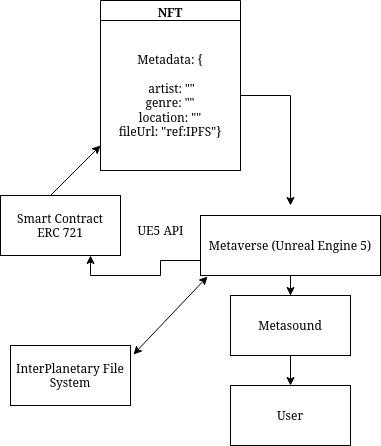
\includegraphics[scale=0.55]{gambar/arsitektur.png}
  % Keterangan gambar yang diinputkan
  \caption{Diagram Arsitektur Sistem}
  % Label referensi dari gambar yang diinputkan
  \label{fig:Architecture}
\end{figure}

\emph{Smart contract} pada arsitektur berguna untuk melakukan operasi-operasi blockchain seperti
memberikan NFT yang berisi metadata dari audio yang sudah disimpan di blockchain sebelumnya.
Untuk file dari audio itu sendiri direferensikan oleh metadata pada NFT tersebut dan akan diambil dari
IPFS menggunakan web3.storage. Metaverse disini diimplementasikan menggunakan Unreal Engine 5 dan menggunakan API
\emph{blockchain} untuk mengeksekusi smart contract. File audio akan diolah oleh metasound dan user akan menerima output audio tersebut.
Untuk deskripsi dari metadata tersebut adalah berupa file JSON dan berikut ini merupakan \emph{interface}-nya

% Contoh input potongan kode dari file
\lstinputlisting[
  language=Python,
  caption={Format data audio.},
  label={lst:formatdataaudio}
]{kode/audioData.json}
Proses perancangan dari arsiktektur sistem yang meliputi IPFS, server, dan blockchain.

\subsection{Proses \emph{generate} NFT dari audio}

Untuk melakukan generate NFT diperlukan proses yang dinamakan Token minting.
Crypto minting adalah sebuah proses komputasi untuk memvalidasi informasi, membuat blok baru dan merekam informasi tersebut ke dalam blockchain.
Dalam proses crypto minting biasanya membutuhkan algoritma konsensus Proof-of-Stake.

\begin{figure} [ht] \centering
  % Nama dari file gambar yang diinputkan
  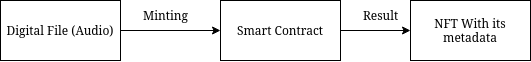
\includegraphics[scale=0.55]{gambar/mintingtoken.png}
  % Keterangan gambar yang diinputkan
  \caption{Diagram Token Minting}
  % Label referensi dari gambar yang diinputkan
  \label{fig:mintingtoken}
\end{figure}

Proof-of-Stake sendiri adalah konsensus yang membantu proses minting seperti bagaimana blok dibuat dan bagaimana data ditambahkan ke blok. Cara kerja crypto minting yaitu koin dicetak (mint) melalui staking di bawah proses Proof-of-Stake. Berbeda halnya dengan Proof-of-Work, Proof-of-Stake tidak memiliki miner. Sebagai gantinya, PoS menggunakan validator. Validator berperan untuk mengamati, juga bertanggung jawab untuk melakukan validasi transaksi dan bekerja untuk menghasilkan blok baru.
Minting adalah proses yang cukup mudah dan terdesentralisasi. Kemudahan dalam proses  minting ini memungkinkan siapa saja untuk membuat token baru tanpa mengharuskan otoritas pusat untuk melakukannya.
Selain itu, ekosistem crypto juga menyediakan berbagai macam token yang diciptakan dengan proses minting, termasuk token aset kripto dan non-fungible token (NFT). Kedua jenis token tersebut tentunya dapat dibuat di berbagai ekosistem blockchain.

\emph{Listing} diatas merupakan \emph{interface} dari metadata yang ditampung di NFT. Semua nilai dari data JSON tersebut
memiliki tipe data yang adalah \emph{string}

\section{Implementasi}

Pembuatan implementasi dari fitur dari aplikasi yang sudah ditentukan melalui tahap
sebelumnya. Tahap ini dilakukan sampai selesai untuk masuk pada tahap validasi. Alokasi
waktu yang ditentukan menyesuaikan dengan pembuatan fitur yang dikerjakan. Pembuatan
implementasi diperkirakan kurang lebih 1 bulan. Implementasi ini termasuk baik pembuatan mini-metaverse
menggunakan \emph{Unreal Engine 5} sebagai sarana untuk melakukan evaluasi dan testing agar keseluruhan sistem dapat terintegrasi.

\subsection{Pembuatan \emph{Smart Contract}}
\emph{Smart Contract} diperlukan untuk membuat perjanjian dengan
berbagai kondisi agar pada \emph{blokchain} bisa mengatur sendiri tanpa
adanya pihak ketika, disini dibuat beberapa kondisi pada
smart contract dalam bentuk kode. Pembuatan smart contract dapat mengacu pada dokumentasi resmi maupun eksternal.
Namun perlu dilakukan modifikasi untuk menyesuaikan dengan desain sistem yang digunakan pada penelitian
ini.

\subsection{Proses \emph{minting} \emph{sound files} menjadi \emph{NFT}}
\emph{Smart contract} yang telah dibuat, kemudian akan dilakukan verifikasi pada \emph{contract} tersebut.

\section{Jadwal Pelaksanaan}

% Ubah tabel berikut sesuai dengan isi dari rencana kerja
\newcommand{\w}{}
\newcommand{\G}{\cellcolor{gray}}
\begin{table}[h!]
  \captionof{table}{Tabel Jadwal Pelaksanaan}
  \label{tbl:timeline}
  \begin{tabular}{|p{3.5cm}|c|c|c|c|c|c|c|c|c|c|c|c|c|c|c|c|}

    \hline
    \multirow{2}{*}{Kegiatan} & \multicolumn{16}{|c|}{Minggu}                                                                       \\
    \cline{2-17}              &
    1                         & 2                             & 3  & 4  & 5  & 6  & 7  & 8  & 9  & 10 & 11 & 12 & 13 & 14 & 15 & 16 \\
    \hline

    % Gunakan \G untuk mengisi sel dan \w untuk mengosongkan sel
    Requirement Analysis      &
    \G                        & \G                            & \w & \w & \w & \w & \w & \w & \w & \w & \w & \w & \w & \w & \w & \w \\
    \hline

    Desain Sistem             &
    \w                        & \w                            & \G & \G & \w & \w & \w & \w & \w & \w & \w & \w & \w & \w & \w & \w \\
    \hline

    Implementasi              &
    \w                        & \w                            & \w & \G & \G & \G & \G & \G & \w & \w & \w & \w & \w & \w & \w & \w \\
    \hline

    Integration Testing       &
    \w                        & \w                            & \w & \w & \w & \w & \w & \w & \G & \G & \w & \w & \w & \w & \w & \w \\
    \hline

    Unit Testing              &
    \w                        & \w                            & \w & \w & \w & \w & \w & \w & \w & \w & \G & \G & \w & \w & \w & \w \\
    \hline

    Evaluasi penelitian       &
    \w                        & \w                            & \w & \w & \w & \w & \w & \w & \w & \w & \w & \w & \G & \G & \G & \G \\
    \hline

    Penyusunan buku           &
    \w                        & \w                            & \w & \w & \w & \w & \G & \G & \G & \G & \G & \G & \G & \G & \G & \G \\
    \hline
  \end{tabular}
\end{table}


% Daftar pustaka
\chapter*{DAFTAR PUSTAKA}
\addcontentsline{toc}{chapter}{DAFTAR PUSTAKA}
\renewcommand\refname{}
\vspace{2ex}
\renewcommand{\bibname}{}
\begingroup
\def\chapter*#1{}
\printbibliography
\endgroup


\end{document}
